% 2011 年江西卷文科第 10 题：凸轮滚动时最高点与中心点的轨迹。
% 来源 PDF：普通高考/2011/2011江西文.pdf，SHA-256 cfb2f18956d0fea24770d3a18e2cc1f32d58b06a4c74b29f83515f64611b0b1f。
% 原页：第 1 页第 2 栏中部，书页码 679。上图为凸轮示意；下排 A—D 为选项（示意）。
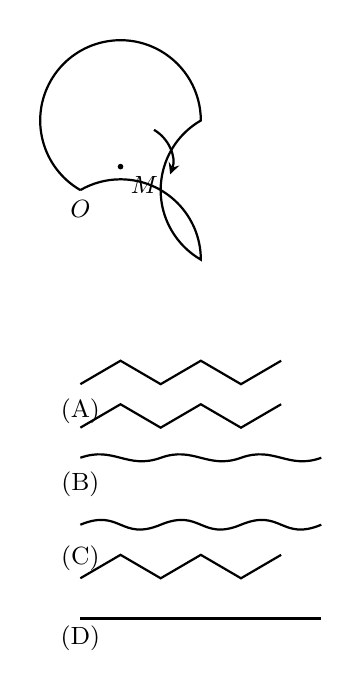
\begin{tikzpicture}[>=stealth, semithick, font=\small, scale=0.85]
  % 凸轮示意（三段等弧围成的圆角三角形）
  \draw[thick] (0,0) arc (240:0:1.2) arc (120:240:1.2) arc (0:120:1.2);
  \fill (0.6,0.35) circle (1.2pt) node[below right] {$M$};
  \node[below] at (0,0) {$O$};
  \draw[->, thick] (1.1,0.9) arc (60:-20:0.55);
  % 选项
  \begin{scope}[yshift=-2.9cm]
    \draw[thick] (0,0) -- (0.6,0.35) -- (1.2,0) -- (1.8,0.35) -- (2.4,0) -- (3.0,0.35);
    \node at (0,-0.4) {(A)};
  \end{scope}
  \begin{scope}[yshift=-4.0cm]
    \draw[thick] (0,0.45) -- (0.6,0.8) -- (1.2,0.45) -- (1.8,0.8) -- (2.4,0.45) -- (3.0,0.8);
    \draw[thick] (0,0) .. controls (0.5,0.18) and (0.7,-0.18) .. (1.2,0) .. controls (1.7,0.18) and (1.9,-0.18) .. (2.4,0) .. controls (2.9,0.18) and (3.1,-0.18) .. (3.6,0);
    \node at (0,-0.4) {(B)};
  \end{scope}
  \begin{scope}[yshift=-5.3cm]
    \draw[thick] (0,0.3) .. controls (0.6,0.55) and (0.6,0.05) .. (1.2,0.3) .. controls (1.8,0.55) and (1.8,0.05) .. (2.4,0.3) .. controls (3.0,0.55) and (3.0,0.05) .. (3.6,0.3);
    \node at (0,-0.2) {(C)};
  \end{scope}
  \begin{scope}[yshift=-6.4cm]
    \draw[thick] (0,0.6) -- (0.6,0.95) -- (1.2,0.6) -- (1.8,0.95) -- (2.4,0.6) -- (3.0,0.95);
    \draw[thick] (0,0)--(3.6,0);
    \node at (0,-0.3) {(D)};
  \end{scope}
\end{tikzpicture}
